\documentclass[twoside]{book}

% Packages required by doxygen
\usepackage{fixltx2e}
\usepackage{calc}
\usepackage{doxygen}
\usepackage{graphicx}
\usepackage[utf8]{inputenc}
\usepackage{makeidx}
\usepackage{multicol}
\usepackage{multirow}
\PassOptionsToPackage{warn}{textcomp}
\usepackage{textcomp}
\usepackage[nointegrals]{wasysym}
\usepackage[table]{xcolor}

% NLS support packages
\usepackage[french]{babel}

% Font selection
\usepackage[T1]{fontenc}
\usepackage{mathptmx}
\usepackage[scaled=.90]{helvet}
\usepackage{courier}
\usepackage{amssymb}
\usepackage{sectsty}
\renewcommand{\familydefault}{\sfdefault}
\allsectionsfont{%
  \fontseries{bc}\selectfont%
  \color{darkgray}%
}
\renewcommand{\DoxyLabelFont}{%
  \fontseries{bc}\selectfont%
  \color{darkgray}%
}
\newcommand{\+}{\discretionary{\mbox{\scriptsize$\hookleftarrow$}}{}{}}

% Page & text layout
\usepackage{geometry}
\geometry{%
  a4paper,%
  top=2.5cm,%
  bottom=2.5cm,%
  left=2.5cm,%
  right=2.5cm%
}
\tolerance=750
\hfuzz=15pt
\hbadness=750
\setlength{\emergencystretch}{15pt}
\setlength{\parindent}{0cm}
\setlength{\parskip}{0.2cm}
\makeatletter
\renewcommand{\paragraph}{%
  \@startsection{paragraph}{4}{0ex}{-1.0ex}{1.0ex}{%
    \normalfont\normalsize\bfseries\SS@parafont%
  }%
}
\renewcommand{\subparagraph}{%
  \@startsection{subparagraph}{5}{0ex}{-1.0ex}{1.0ex}{%
    \normalfont\normalsize\bfseries\SS@subparafont%
  }%
}
\makeatother

% Headers & footers
\usepackage{fancyhdr}
\pagestyle{fancyplain}
\fancyhead[LE]{\fancyplain{}{\bfseries\thepage}}
\fancyhead[CE]{\fancyplain{}{}}
\fancyhead[RE]{\fancyplain{}{\bfseries\leftmark}}
\fancyhead[LO]{\fancyplain{}{\bfseries\rightmark}}
\fancyhead[CO]{\fancyplain{}{}}
\fancyhead[RO]{\fancyplain{}{\bfseries\thepage}}
\fancyfoot[LE]{\fancyplain{}{}}
\fancyfoot[CE]{\fancyplain{}{}}
\fancyfoot[RE]{\fancyplain{}{\bfseries\scriptsize Généré le Mercredi 10 Juin 2015 15\+:52\+:10 pour D\+P\+Zip par Doxygen }}
\fancyfoot[LO]{\fancyplain{}{\bfseries\scriptsize Généré le Mercredi 10 Juin 2015 15\+:52\+:10 pour D\+P\+Zip par Doxygen }}
\fancyfoot[CO]{\fancyplain{}{}}
\fancyfoot[RO]{\fancyplain{}{}}
\renewcommand{\footrulewidth}{0.4pt}
\renewcommand{\chaptermark}[1]{%
  \markboth{#1}{}%
}
\renewcommand{\sectionmark}[1]{%
  \markright{\thesection\ #1}%
}

% Indices & bibliography
\usepackage{natbib}
\usepackage[titles]{tocloft}
\setcounter{tocdepth}{3}
\setcounter{secnumdepth}{5}
\makeindex

% Hyperlinks (required, but should be loaded last)
\usepackage{ifpdf}
\ifpdf
  \usepackage[pdftex,pagebackref=true]{hyperref}
\else
  \usepackage[ps2pdf,pagebackref=true]{hyperref}
\fi
\hypersetup{%
  colorlinks=true,%
  linkcolor=blue,%
  citecolor=blue,%
  unicode%
}

% Custom commands
\newcommand{\clearemptydoublepage}{%
  \newpage{\pagestyle{empty}\cleardoublepage}%
}


%===== C O N T E N T S =====

\begin{document}

% Titlepage & ToC
\hypersetup{pageanchor=false,
             bookmarks=true,
             bookmarksnumbered=true,
             pdfencoding=unicode
            }
\pagenumbering{roman}
\begin{titlepage}
\vspace*{7cm}
\begin{center}%
{\Large D\+P\+Zip }\\
\vspace*{1cm}
{\large Généré par Doxygen 1.8.8}\\
\vspace*{0.5cm}
{\small Mercredi 10 Juin 2015 15:52:10}\\
\end{center}
\end{titlepage}
\clearemptydoublepage
\tableofcontents
\clearemptydoublepage
\pagenumbering{arabic}
\hypersetup{pageanchor=true}

%--- Begin generated contents ---
\chapter{D\+P\+Zip Documentation}
\label{index}\hypertarget{index}{}\hypertarget{index_author_sec}{}\section{Author}\label{index_author_sec}
Paul F\+I\+O\+R\+E\+N\+T\+I\+N\+O -\/ Damien M\+A\+U\+R\+I\+N\hypertarget{index_date_sec}{}\section{Date}\label{index_date_sec}
Juin 2015\hypertarget{index_summary_sec}{}\section{Summary}\label{index_summary_sec}
\hyperlink{class_d_p_zip}{D\+P\+Zip} est un compresseur/décompresseur de fichier multithread 
\chapter{D\+P\+Zip}
\label{md__r_e_a_d_m_e}
\hypertarget{md__r_e_a_d_m_e}{}
Projet C++ 
\chapter{Index hiérarchique}
\section{Hiérarchie des classes}
Cette liste d'héritage est classée approximativement par ordre alphabétique \+:\begin{DoxyCompactList}
\item \contentsline{section}{Data\+Buffer}{\pageref{class_data_buffer}}{}
\item \contentsline{section}{Data\+Pool$<$ T $>$}{\pageref{class_data_pool}}{}
\item \contentsline{section}{Data\+Pool$<$ Data\+Buffer $>$}{\pageref{class_data_pool}}{}
\item \contentsline{section}{Data\+Pool$<$ Q\+String $>$}{\pageref{class_data_pool}}{}
\item \contentsline{section}{D\+P\+Zip}{\pageref{class_d_p_zip}}{}
\item Q\+Thread\begin{DoxyCompactList}
\item \contentsline{section}{Reader}{\pageref{class_reader}}{}
\item \contentsline{section}{U\+C\+File\+Writer}{\pageref{class_u_c_file_writer}}{}
\item \contentsline{section}{Unzipper}{\pageref{class_unzipper}}{}
\item \contentsline{section}{Writer}{\pageref{class_writer}}{}
\item \contentsline{section}{Zipper}{\pageref{class_zipper}}{}
\end{DoxyCompactList}
\end{DoxyCompactList}

\chapter{Index des classes}
\section{Liste des classes}
Liste des classes, structures, unions et interfaces avec une brève description \+:\begin{DoxyCompactList}
\item\contentsline{section}{\hyperlink{class_data_buffer}{Data\+Buffer} \\*La classe \hyperlink{class_data_buffer}{Data\+Buffer} représente un fichier de données qu'il soit compressé ou à compresser il sera stocké de la même manière dans cette structure }{\pageref{class_data_buffer}}{}
\item\contentsline{section}{\hyperlink{class_data_pool}{Data\+Pool$<$ T $>$} \\*La classe \hyperlink{class_data_pool}{Data\+Pool} est une structure de donnée qui peut contenir des données de type spécifié par $<$template T$>$ Toutes les méthodes de cette classe sont thread-\/safe }{\pageref{class_data_pool}}{}
\item\contentsline{section}{\hyperlink{class_d_p_zip}{D\+P\+Zip} \\*La classe \hyperlink{class_d_p_zip}{D\+P\+Zip} est la classe principale de l'application elle permet la compression et la décompression de fichiers }{\pageref{class_d_p_zip}}{}
\item\contentsline{section}{\hyperlink{class_reader}{Reader} \\*La classe \hyperlink{class_reader}{Reader} permet de désérialiser le contenu d'un fichier .ecf et de stocker les objets obtenus (compressés) dans un \hyperlink{class_data_pool}{Data\+Pool} }{\pageref{class_reader}}{}
\item\contentsline{section}{\hyperlink{class_u_c_file_writer}{U\+C\+File\+Writer} \\*La classe \hyperlink{class_u_c_file_writer}{U\+C\+File\+Writer} permet d'écrire sur le disque tous les fichiers d'un \hyperlink{class_data_pool}{Data\+Pool} passé en paramètre }{\pageref{class_u_c_file_writer}}{}
\item\contentsline{section}{\hyperlink{class_unzipper}{Unzipper} \\*La classe \hyperlink{class_unzipper}{Unzipper} récupère des données compressées d'un \hyperlink{class_data_pool}{Data\+Pool}, les décompresse et les ajoute à un second \hyperlink{class_data_pool}{Data\+Pool} }{\pageref{class_unzipper}}{}
\item\contentsline{section}{\hyperlink{class_writer}{Writer} \\*La classe \hyperlink{class_writer}{Writer} écrit un fichier .ecf à partir d'un \hyperlink{class_data_pool}{Data\+Pool} de donées compressées }{\pageref{class_writer}}{}
\item\contentsline{section}{\hyperlink{class_zipper}{Zipper} \\*La classe \hyperlink{class_zipper}{Zipper} permet de compresser les données d'un \hyperlink{class_data_pool}{Data\+Pool} et de les stocker dans un second \hyperlink{class_data_pool}{Data\+Pool} }{\pageref{class_zipper}}{}
\end{DoxyCompactList}

\chapter{Documentation des classes}
\hypertarget{class_data_buffer}{\section{Référence de la classe Data\+Buffer}
\label{class_data_buffer}\index{Data\+Buffer@{Data\+Buffer}}
}


La classe \hyperlink{class_data_buffer}{Data\+Buffer} représente un fichier de données qu'il soit compressé ou à compresser il sera stocké de la même manière dans cette structure.  




{\ttfamily \#include $<$databuffer.\+h$>$}

\subsection*{Fonctions membres publiques}
\begin{DoxyCompactItemize}
\item 
\hypertarget{class_data_buffer_a83f823dc058fe550713806bb49dd9651}{\hyperlink{class_data_buffer_a83f823dc058fe550713806bb49dd9651}{Data\+Buffer} ()}\label{class_data_buffer_a83f823dc058fe550713806bb49dd9651}

\begin{DoxyCompactList}\small\item\em \hyperlink{class_data_buffer}{Data\+Buffer} contruit un nouveau fichier en mémoire. \end{DoxyCompactList}\item 
void \hyperlink{class_data_buffer_a020c2a9e6f84f77fb7424845ae532da4}{set\+File\+Name} (const Q\+String \&file\+Name)
\begin{DoxyCompactList}\small\item\em set\+File\+Name définit le nom du fichier \end{DoxyCompactList}\item 
const Q\+String \hyperlink{class_data_buffer_ac63e75c4e19e45b2d70f1879c6f7e34e}{get\+File\+Name} ()
\begin{DoxyCompactList}\small\item\em get\+File\+Name retourne le nom du fichier \end{DoxyCompactList}\item 
void \hyperlink{class_data_buffer_ada256ca15ccca7e92c733bd45c939741}{set\+Data} (const Q\+Byte\+Array \&data)
\begin{DoxyCompactList}\small\item\em set\+Data stocke les données brutes du fichier \end{DoxyCompactList}\item 
const Q\+Byte\+Array \hyperlink{class_data_buffer_a37aa198c3266ac7fe4925157d6bfd0d1}{get\+Data} ()
\begin{DoxyCompactList}\small\item\em get\+Data retourne les données brutes du fichier \end{DoxyCompactList}\item 
void \hyperlink{class_data_buffer_a4c865943b6b4c3f802fefbdefdfc912a}{read} (Q\+Data\+Stream \&stream)
\begin{DoxyCompactList}\small\item\em read récupère et désérialise un objet \hyperlink{class_data_buffer}{Data\+Buffer} contenu dans le Q\+Data\+Stream passé en paramètre \end{DoxyCompactList}\item 
void \hyperlink{class_data_buffer_a859adb76758375b3aacffc42702277f3}{write} (Q\+Data\+Stream \&stream)
\begin{DoxyCompactList}\small\item\em write sérialise un objet \hyperlink{class_data_buffer}{Data\+Buffer} dans un Q\+Data\+Stream passé en paramètre \end{DoxyCompactList}\item 
void \hyperlink{class_data_buffer_a4cb04bf885a20c93622360b9f2615ba2}{write\+Raw\+Data} (Q\+Data\+Stream \&stream)
\begin{DoxyCompactList}\small\item\em write écrit les données brutes dans un Q\+Data\+Stream Se différencie de write par le fait qu'elle écrive directement les données brutes et non l'objet sérialisé \end{DoxyCompactList}\end{DoxyCompactItemize}


\subsection{Description détaillée}
La classe \hyperlink{class_data_buffer}{Data\+Buffer} représente un fichier de données qu'il soit compressé ou à compresser il sera stocké de la même manière dans cette structure. 

\subsection{Documentation des fonctions membres}
\hypertarget{class_data_buffer_a37aa198c3266ac7fe4925157d6bfd0d1}{\index{Data\+Buffer@{Data\+Buffer}!get\+Data@{get\+Data}}
\index{get\+Data@{get\+Data}!Data\+Buffer@{Data\+Buffer}}
\subsubsection[{get\+Data}]{\setlength{\rightskip}{0pt plus 5cm}const Q\+Byte\+Array Data\+Buffer\+::get\+Data (
\begin{DoxyParamCaption}
{}
\end{DoxyParamCaption}
)}}\label{class_data_buffer_a37aa198c3266ac7fe4925157d6bfd0d1}


get\+Data retourne les données brutes du fichier 

\begin{DoxyReturn}{Renvoie}

\end{DoxyReturn}
\hypertarget{class_data_buffer_ac63e75c4e19e45b2d70f1879c6f7e34e}{\index{Data\+Buffer@{Data\+Buffer}!get\+File\+Name@{get\+File\+Name}}
\index{get\+File\+Name@{get\+File\+Name}!Data\+Buffer@{Data\+Buffer}}
\subsubsection[{get\+File\+Name}]{\setlength{\rightskip}{0pt plus 5cm}const Q\+String Data\+Buffer\+::get\+File\+Name (
\begin{DoxyParamCaption}
{}
\end{DoxyParamCaption}
)}}\label{class_data_buffer_ac63e75c4e19e45b2d70f1879c6f7e34e}


get\+File\+Name retourne le nom du fichier 

\begin{DoxyReturn}{Renvoie}

\end{DoxyReturn}
\hypertarget{class_data_buffer_a4c865943b6b4c3f802fefbdefdfc912a}{\index{Data\+Buffer@{Data\+Buffer}!read@{read}}
\index{read@{read}!Data\+Buffer@{Data\+Buffer}}
\subsubsection[{read}]{\setlength{\rightskip}{0pt plus 5cm}void Data\+Buffer\+::read (
\begin{DoxyParamCaption}
\item[{Q\+Data\+Stream \&}]{stream}
\end{DoxyParamCaption}
)}}\label{class_data_buffer_a4c865943b6b4c3f802fefbdefdfc912a}


read récupère et désérialise un objet \hyperlink{class_data_buffer}{Data\+Buffer} contenu dans le Q\+Data\+Stream passé en paramètre 


\begin{DoxyParams}{Paramètres}
{\em stream} & Q\+Data\+Stream contenant les Buffers sérialisés \\
\hline
\end{DoxyParams}
\hypertarget{class_data_buffer_ada256ca15ccca7e92c733bd45c939741}{\index{Data\+Buffer@{Data\+Buffer}!set\+Data@{set\+Data}}
\index{set\+Data@{set\+Data}!Data\+Buffer@{Data\+Buffer}}
\subsubsection[{set\+Data}]{\setlength{\rightskip}{0pt plus 5cm}void Data\+Buffer\+::set\+Data (
\begin{DoxyParamCaption}
\item[{const Q\+Byte\+Array \&}]{data}
\end{DoxyParamCaption}
)}}\label{class_data_buffer_ada256ca15ccca7e92c733bd45c939741}


set\+Data stocke les données brutes du fichier 


\begin{DoxyParams}{Paramètres}
{\em data} & données du fichier \\
\hline
\end{DoxyParams}
\hypertarget{class_data_buffer_a020c2a9e6f84f77fb7424845ae532da4}{\index{Data\+Buffer@{Data\+Buffer}!set\+File\+Name@{set\+File\+Name}}
\index{set\+File\+Name@{set\+File\+Name}!Data\+Buffer@{Data\+Buffer}}
\subsubsection[{set\+File\+Name}]{\setlength{\rightskip}{0pt plus 5cm}void Data\+Buffer\+::set\+File\+Name (
\begin{DoxyParamCaption}
\item[{const Q\+String \&}]{file\+Name}
\end{DoxyParamCaption}
)}}\label{class_data_buffer_a020c2a9e6f84f77fb7424845ae532da4}


set\+File\+Name définit le nom du fichier 


\begin{DoxyParams}{Paramètres}
{\em file\+Name} & le nom du fichier \\
\hline
\end{DoxyParams}
\hypertarget{class_data_buffer_a859adb76758375b3aacffc42702277f3}{\index{Data\+Buffer@{Data\+Buffer}!write@{write}}
\index{write@{write}!Data\+Buffer@{Data\+Buffer}}
\subsubsection[{write}]{\setlength{\rightskip}{0pt plus 5cm}void Data\+Buffer\+::write (
\begin{DoxyParamCaption}
\item[{Q\+Data\+Stream \&}]{stream}
\end{DoxyParamCaption}
)}}\label{class_data_buffer_a859adb76758375b3aacffc42702277f3}


write sérialise un objet \hyperlink{class_data_buffer}{Data\+Buffer} dans un Q\+Data\+Stream passé en paramètre 


\begin{DoxyParams}{Paramètres}
{\em stream} & Q\+Data\+Stream cible \\
\hline
\end{DoxyParams}
\hypertarget{class_data_buffer_a4cb04bf885a20c93622360b9f2615ba2}{\index{Data\+Buffer@{Data\+Buffer}!write\+Raw\+Data@{write\+Raw\+Data}}
\index{write\+Raw\+Data@{write\+Raw\+Data}!Data\+Buffer@{Data\+Buffer}}
\subsubsection[{write\+Raw\+Data}]{\setlength{\rightskip}{0pt plus 5cm}void Data\+Buffer\+::write\+Raw\+Data (
\begin{DoxyParamCaption}
\item[{Q\+Data\+Stream \&}]{stream}
\end{DoxyParamCaption}
)}}\label{class_data_buffer_a4cb04bf885a20c93622360b9f2615ba2}


write écrit les données brutes dans un Q\+Data\+Stream Se différencie de write par le fait qu'elle écrive directement les données brutes et non l'objet sérialisé 


\begin{DoxyParams}{Paramètres}
{\em stream} & Q\+Data\+Stream cible \\
\hline
\end{DoxyParams}


La documentation de cette classe a été générée à partir des fichiers suivants \+:\begin{DoxyCompactItemize}
\item 
databuffer.\+h\item 
databuffer.\+cpp\end{DoxyCompactItemize}

\hypertarget{class_data_pool}{\section{Référence du modèle de la classe Data\+Pool$<$ T $>$}
\label{class_data_pool}\index{Data\+Pool$<$ T $>$@{Data\+Pool$<$ T $>$}}
}


La classe \hyperlink{class_data_pool}{Data\+Pool} est une structure de donnée qui peut contenir des données de type spécifié par $<$template T$>$ Toutes les méthodes de cette classe sont thread-\/safe.  




{\ttfamily \#include $<$datapool.\+h$>$}

\subsection*{Fonctions membres publiques}
\begin{DoxyCompactItemize}
\item 
\hypertarget{class_data_pool_a0e93f42b7be1b1ffa03a79a9220cca2c}{\hyperlink{class_data_pool_a0e93f42b7be1b1ffa03a79a9220cca2c}{Data\+Pool} ()}\label{class_data_pool_a0e93f42b7be1b1ffa03a79a9220cca2c}

\begin{DoxyCompactList}\small\item\em \hyperlink{class_data_pool}{Data\+Pool} contruit un nouveau \hyperlink{class_data_pool}{Data\+Pool} de données thread-\/safe. \end{DoxyCompactList}\item 
void \hyperlink{class_data_pool_af87b1ba98e148de273975fbbf2d6eb49}{put} (T \&element)
\begin{DoxyCompactList}\small\item\em put ajoute un nouvel élément au \hyperlink{class_data_pool}{Data\+Pool} thread-\/safe \end{DoxyCompactList}\item 
Q\+Pair$<$ bool, T $>$ \hyperlink{class_data_pool_a4b46a347e1fa6b3eeafed9d77eb7eaa7}{try\+Get} ()
\begin{DoxyCompactList}\small\item\em trye\+Get tente de récupérer un élément du \hyperlink{class_data_pool}{Data\+Pool} thread-\/safe \end{DoxyCompactList}\item 
int \hyperlink{class_data_pool_a0ee10a72e547a3de6c24a3997a961c85}{count} ()
\begin{DoxyCompactList}\small\item\em count retourne le nombre d'éléments encore présents dans le \hyperlink{class_data_pool}{Data\+Pool} thread-\/safe \end{DoxyCompactList}\item 
\hypertarget{class_data_pool_a0760141bdcfcbd2d9992a5ccaf064ce8}{void \hyperlink{class_data_pool_a0760141bdcfcbd2d9992a5ccaf064ce8}{done} ()}\label{class_data_pool_a0760141bdcfcbd2d9992a5ccaf064ce8}

\begin{DoxyCompactList}\small\item\em done signale au \hyperlink{class_data_pool}{Data\+Pool} qu'aucun nouvel élément sera ajouté permet de libérer la Q\+Wait\+Condition \end{DoxyCompactList}\end{DoxyCompactItemize}


\subsection{Description détaillée}
\subsubsection*{template$<$typename T$>$class Data\+Pool$<$ T $>$}

La classe \hyperlink{class_data_pool}{Data\+Pool} est une structure de donnée qui peut contenir des données de type spécifié par $<$template T$>$ Toutes les méthodes de cette classe sont thread-\/safe. 

\subsection{Documentation des fonctions membres}
\hypertarget{class_data_pool_a0ee10a72e547a3de6c24a3997a961c85}{\index{Data\+Pool@{Data\+Pool}!count@{count}}
\index{count@{count}!Data\+Pool@{Data\+Pool}}
\subsubsection[{count}]{\setlength{\rightskip}{0pt plus 5cm}template$<$typename T $>$ int {\bf Data\+Pool}$<$ T $>$\+::count (
\begin{DoxyParamCaption}
{}
\end{DoxyParamCaption}
)}}\label{class_data_pool_a0ee10a72e547a3de6c24a3997a961c85}


count retourne le nombre d'éléments encore présents dans le \hyperlink{class_data_pool}{Data\+Pool} thread-\/safe 

\begin{DoxyReturn}{Renvoie}
nombre d'éléments contenus dans le pool 
\end{DoxyReturn}
\hypertarget{class_data_pool_af87b1ba98e148de273975fbbf2d6eb49}{\index{Data\+Pool@{Data\+Pool}!put@{put}}
\index{put@{put}!Data\+Pool@{Data\+Pool}}
\subsubsection[{put}]{\setlength{\rightskip}{0pt plus 5cm}template$<$typename T$>$ void {\bf Data\+Pool}$<$ T $>$\+::put (
\begin{DoxyParamCaption}
\item[{T \&}]{element}
\end{DoxyParamCaption}
)}}\label{class_data_pool_af87b1ba98e148de273975fbbf2d6eb49}


put ajoute un nouvel élément au \hyperlink{class_data_pool}{Data\+Pool} thread-\/safe 


\begin{DoxyParams}{Paramètres}
{\em element} & élément à ajouter \\
\hline
\end{DoxyParams}
\hypertarget{class_data_pool_a4b46a347e1fa6b3eeafed9d77eb7eaa7}{\index{Data\+Pool@{Data\+Pool}!try\+Get@{try\+Get}}
\index{try\+Get@{try\+Get}!Data\+Pool@{Data\+Pool}}
\subsubsection[{try\+Get}]{\setlength{\rightskip}{0pt plus 5cm}template$<$typename T $>$ Q\+Pair$<$ bool, T $>$ {\bf Data\+Pool}$<$ T $>$\+::try\+Get (
\begin{DoxyParamCaption}
{}
\end{DoxyParamCaption}
)}}\label{class_data_pool_a4b46a347e1fa6b3eeafed9d77eb7eaa7}


trye\+Get tente de récupérer un élément du \hyperlink{class_data_pool}{Data\+Pool} thread-\/safe 

\begin{DoxyReturn}{Renvoie}
Q\+Pair$<$bool, T$>$~\newline
bool\+: true si l'élément récupéré est valide~\newline
T\+: élément récupéré 
\end{DoxyReturn}


La documentation de cette classe a été générée à partir des fichiers suivants \+:\begin{DoxyCompactItemize}
\item 
datapool.\+h\item 
datapool.\+cpp\end{DoxyCompactItemize}

\hypertarget{class_d_p_zip}{\section{Référence de la classe D\+P\+Zip}
\label{class_d_p_zip}\index{D\+P\+Zip@{D\+P\+Zip}}
}


La classe \hyperlink{class_d_p_zip}{D\+P\+Zip} est la classe principale de l'application elle permet la compression et la décompression de fichiers.  




{\ttfamily \#include $<$dpzip.\+h$>$}

\subsection*{Fonctions membres publiques}
\begin{DoxyCompactItemize}
\item 
\hyperlink{class_d_p_zip_ac6061f1fb5304fa46d2cb036faf513cb}{D\+P\+Zip} (const int num\+Threads)
\begin{DoxyCompactList}\small\item\em \hyperlink{class_d_p_zip}{D\+P\+Zip} contructeur de la classe. \end{DoxyCompactList}\item 
void \hyperlink{class_d_p_zip_a5210127d2033c46124082aaff4d0b389}{compress} (const Q\+String \&folder, const Q\+String \&ecf\+File\+Name, bool compress\+Hidden\+Files=false)
\begin{DoxyCompactList}\small\item\em compress compresse un dossier dans un fichier .ecf \end{DoxyCompactList}\item 
void \hyperlink{class_d_p_zip_a6e0195fe368f40cb232596cf135675e7}{uncompress} (const Q\+String \&ecf\+File\+Name, const Q\+String \&out\+Folder)
\begin{DoxyCompactList}\small\item\em uncompress décompresse un fichier .ecf dans un répertoire donné \end{DoxyCompactList}\end{DoxyCompactItemize}


\subsection{Description détaillée}
La classe \hyperlink{class_d_p_zip}{D\+P\+Zip} est la classe principale de l'application elle permet la compression et la décompression de fichiers. 

\subsection{Documentation des constructeurs et destructeur}
\hypertarget{class_d_p_zip_ac6061f1fb5304fa46d2cb036faf513cb}{\index{D\+P\+Zip@{D\+P\+Zip}!D\+P\+Zip@{D\+P\+Zip}}
\index{D\+P\+Zip@{D\+P\+Zip}!D\+P\+Zip@{D\+P\+Zip}}
\subsubsection[{D\+P\+Zip}]{\setlength{\rightskip}{0pt plus 5cm}D\+P\+Zip\+::\+D\+P\+Zip (
\begin{DoxyParamCaption}
\item[{const int}]{num\+Threads}
\end{DoxyParamCaption}
)}}\label{class_d_p_zip_ac6061f1fb5304fa46d2cb036faf513cb}


\hyperlink{class_d_p_zip}{D\+P\+Zip} contructeur de la classe. 


\begin{DoxyParams}{Paramètres}
{\em num\+Threads} & nombre de threads de zipper ou de unzipper à lancer \\
\hline
\end{DoxyParams}


\subsection{Documentation des fonctions membres}
\hypertarget{class_d_p_zip_a5210127d2033c46124082aaff4d0b389}{\index{D\+P\+Zip@{D\+P\+Zip}!compress@{compress}}
\index{compress@{compress}!D\+P\+Zip@{D\+P\+Zip}}
\subsubsection[{compress}]{\setlength{\rightskip}{0pt plus 5cm}void D\+P\+Zip\+::compress (
\begin{DoxyParamCaption}
\item[{const Q\+String \&}]{folder, }
\item[{const Q\+String \&}]{ecf\+File\+Name, }
\item[{bool}]{compress\+Hidden\+Files = {\ttfamily false}}
\end{DoxyParamCaption}
)}}\label{class_d_p_zip_a5210127d2033c46124082aaff4d0b389}


compress compresse un dossier dans un fichier .ecf 


\begin{DoxyParams}{Paramètres}
{\em folder} & dossier à compresser \\
\hline
{\em ecf\+File\+Name} & fichier .ecf de destination \\
\hline
{\em compress\+Hidden\+Files} & ajouter ou non les fichiers cachés du système d'exploitation à l'archive \\
\hline
\end{DoxyParams}
\hypertarget{class_d_p_zip_a6e0195fe368f40cb232596cf135675e7}{\index{D\+P\+Zip@{D\+P\+Zip}!uncompress@{uncompress}}
\index{uncompress@{uncompress}!D\+P\+Zip@{D\+P\+Zip}}
\subsubsection[{uncompress}]{\setlength{\rightskip}{0pt plus 5cm}void D\+P\+Zip\+::uncompress (
\begin{DoxyParamCaption}
\item[{const Q\+String \&}]{ecf\+File\+Name, }
\item[{const Q\+String \&}]{out\+Folder}
\end{DoxyParamCaption}
)}}\label{class_d_p_zip_a6e0195fe368f40cb232596cf135675e7}


uncompress décompresse un fichier .ecf dans un répertoire donné 


\begin{DoxyParams}{Paramètres}
{\em ecf\+File\+Name} & fichier à décompresser \\
\hline
{\em out\+Folder} & répertoire de destination, s'il n'existe pas il sera créé \\
\hline
\end{DoxyParams}


La documentation de cette classe a été générée à partir des fichiers suivants \+:\begin{DoxyCompactItemize}
\item 
dpzip.\+h\item 
dpzip.\+cpp\end{DoxyCompactItemize}

\hypertarget{class_reader}{\section{Référence de la classe Reader}
\label{class_reader}\index{Reader@{Reader}}
}


La classe \hyperlink{class_reader}{Reader} permet de désérialiser le contenu d'un fichier .ecf et de stocker les objets obtenus (compressés) dans un \hyperlink{class_data_pool}{Data\+Pool}.  




{\ttfamily \#include $<$reader.\+h$>$}

Graphe d'héritage de Reader\+:\begin{figure}[H]
\begin{center}
\leavevmode
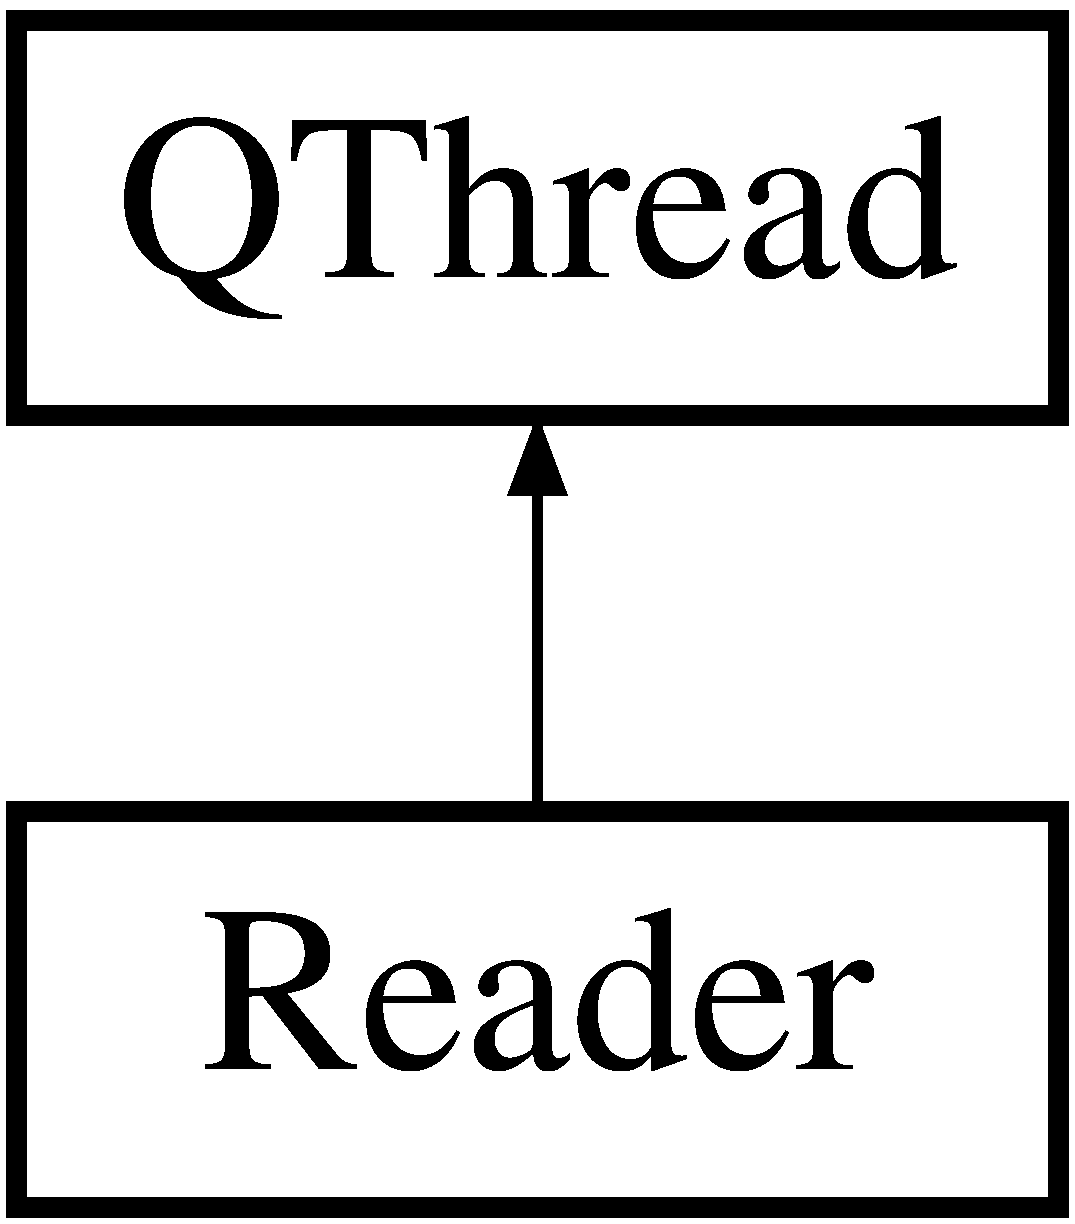
\includegraphics[height=2.000000cm]{class_reader}
\end{center}
\end{figure}
\subsection*{Fonctions membres publiques}
\begin{DoxyCompactItemize}
\item 
\hyperlink{class_reader_a85ffbb6feed009ea992370b829c1d4c5}{Reader} (const Q\+String ecf\+File\+Name, \hyperlink{class_data_pool}{Data\+Pool}$<$ \hyperlink{class_data_buffer}{Data\+Buffer} $>$ \&\+\_\+zipped\+Files\+Pool)
\begin{DoxyCompactList}\small\item\em \hyperlink{class_reader}{Reader} constructeur de la classe. \end{DoxyCompactList}\item 
\hypertarget{class_reader_aac4ef17c2ee8e7a45820dc23a7f92d3e}{virtual void {\bfseries run} ()}\label{class_reader_aac4ef17c2ee8e7a45820dc23a7f92d3e}

\end{DoxyCompactItemize}


\subsection{Description détaillée}
La classe \hyperlink{class_reader}{Reader} permet de désérialiser le contenu d'un fichier .ecf et de stocker les objets obtenus (compressés) dans un \hyperlink{class_data_pool}{Data\+Pool}. 

\subsection{Documentation des constructeurs et destructeur}
\hypertarget{class_reader_a85ffbb6feed009ea992370b829c1d4c5}{\index{Reader@{Reader}!Reader@{Reader}}
\index{Reader@{Reader}!Reader@{Reader}}
\subsubsection[{Reader}]{\setlength{\rightskip}{0pt plus 5cm}Reader\+::\+Reader (
\begin{DoxyParamCaption}
\item[{const Q\+String}]{ecf\+File\+Name, }
\item[{{\bf Data\+Pool}$<$ {\bf Data\+Buffer} $>$ \&}]{\+\_\+zipped\+Files\+Pool}
\end{DoxyParamCaption}
)}}\label{class_reader_a85ffbb6feed009ea992370b829c1d4c5}


\hyperlink{class_reader}{Reader} constructeur de la classe. 


\begin{DoxyParams}{Paramètres}
{\em ecf\+File\+Name} & fichier à désérialiser \\
\hline
{\em \+\_\+zipped\+Files\+Pool} & \hyperlink{class_data_pool}{Data\+Pool} d'objets désérialisés (mais compressées) \\
\hline
\end{DoxyParams}


La documentation de cette classe a été générée à partir des fichiers suivants \+:\begin{DoxyCompactItemize}
\item 
reader.\+h\item 
reader.\+cpp\end{DoxyCompactItemize}

\hypertarget{class_u_c_file_writer}{\section{Référence de la classe U\+C\+File\+Writer}
\label{class_u_c_file_writer}\index{U\+C\+File\+Writer@{U\+C\+File\+Writer}}
}


La classe \hyperlink{class_u_c_file_writer}{U\+C\+File\+Writer} permet d'écrire sur le disque tous les fichiers d'un \hyperlink{class_data_pool}{Data\+Pool} passé en paramètre.  




{\ttfamily \#include $<$ucfilewriter.\+h$>$}

Graphe d'héritage de U\+C\+File\+Writer\+:\begin{figure}[H]
\begin{center}
\leavevmode
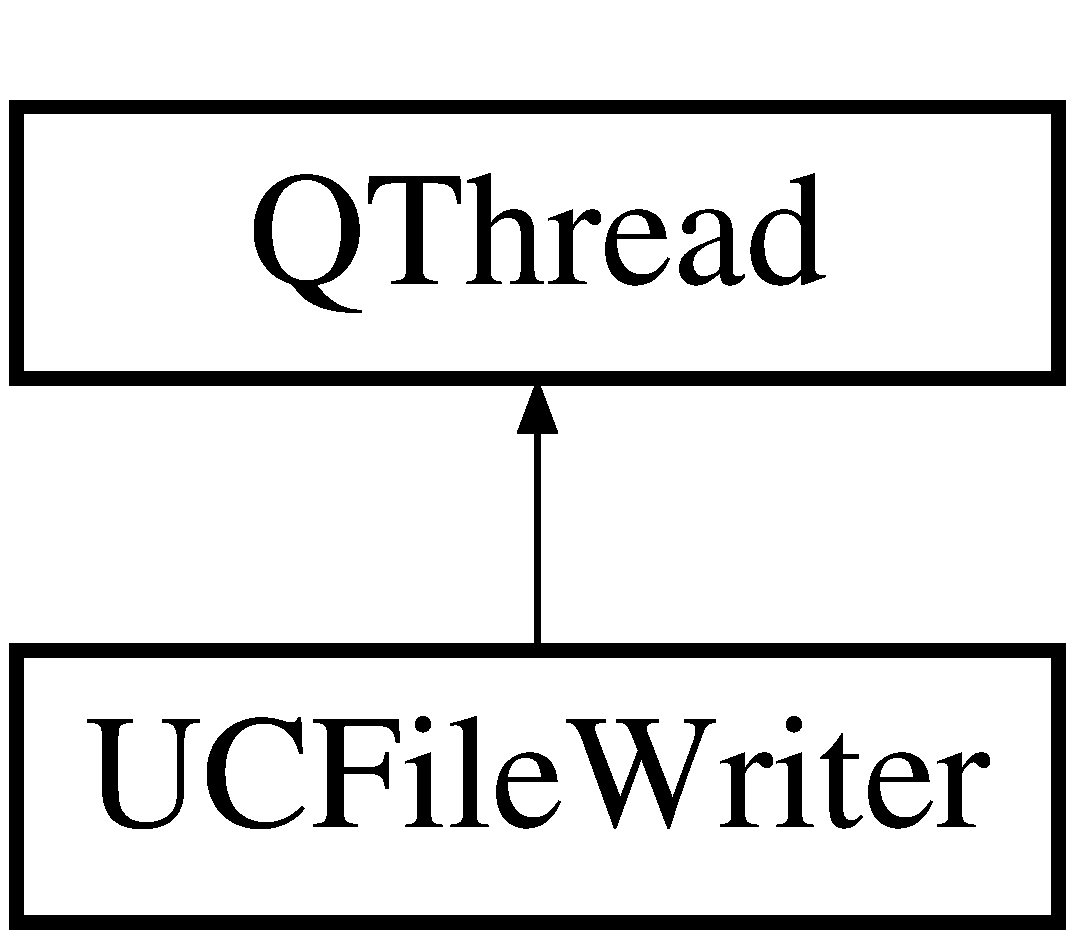
\includegraphics[height=2.000000cm]{class_u_c_file_writer}
\end{center}
\end{figure}
\subsection*{Fonctions membres publiques}
\begin{DoxyCompactItemize}
\item 
\hyperlink{class_u_c_file_writer_a5a3d8600c1b5b5063500021fe9df15b3}{U\+C\+File\+Writer} (\hyperlink{class_data_pool}{Data\+Pool}$<$ \hyperlink{class_data_buffer}{Data\+Buffer} $>$ \&unzipped\+Files\+Pool, const Q\+String \&dest\+Folder)
\begin{DoxyCompactList}\small\item\em \hyperlink{class_u_c_file_writer}{U\+C\+File\+Writer} constructeur de la classe. \end{DoxyCompactList}\item 
\hypertarget{class_u_c_file_writer_a707cdd9f57aef4df03fd3e82a5820836}{virtual void {\bfseries run} ()}\label{class_u_c_file_writer_a707cdd9f57aef4df03fd3e82a5820836}

\end{DoxyCompactItemize}


\subsection{Description détaillée}
La classe \hyperlink{class_u_c_file_writer}{U\+C\+File\+Writer} permet d'écrire sur le disque tous les fichiers d'un \hyperlink{class_data_pool}{Data\+Pool} passé en paramètre. 

\subsection{Documentation des constructeurs et destructeur}
\hypertarget{class_u_c_file_writer_a5a3d8600c1b5b5063500021fe9df15b3}{\index{U\+C\+File\+Writer@{U\+C\+File\+Writer}!U\+C\+File\+Writer@{U\+C\+File\+Writer}}
\index{U\+C\+File\+Writer@{U\+C\+File\+Writer}!U\+C\+File\+Writer@{U\+C\+File\+Writer}}
\subsubsection[{U\+C\+File\+Writer}]{\setlength{\rightskip}{0pt plus 5cm}U\+C\+File\+Writer\+::\+U\+C\+File\+Writer (
\begin{DoxyParamCaption}
\item[{{\bf Data\+Pool}$<$ {\bf Data\+Buffer} $>$ \&}]{unzipped\+Files\+Pool, }
\item[{const Q\+String \&}]{dest\+Folder}
\end{DoxyParamCaption}
)}}\label{class_u_c_file_writer_a5a3d8600c1b5b5063500021fe9df15b3}


\hyperlink{class_u_c_file_writer}{U\+C\+File\+Writer} constructeur de la classe. 


\begin{DoxyParams}{Paramètres}
{\em unzipped\+Files\+Pool} & \hyperlink{class_data_pool}{Data\+Pool} de données décompressées à écrire \\
\hline
{\em dest\+Folder} & dossier racine de destination (chaque fichier contient son path relatif à ce dossier) \\
\hline
\end{DoxyParams}


La documentation de cette classe a été générée à partir des fichiers suivants \+:\begin{DoxyCompactItemize}
\item 
ucfilewriter.\+h\item 
ucfilewriter.\+cpp\end{DoxyCompactItemize}

\hypertarget{class_unzipper}{\section{Référence de la classe Unzipper}
\label{class_unzipper}\index{Unzipper@{Unzipper}}
}


La classe \hyperlink{class_unzipper}{Unzipper} récupère des données compressées d'un \hyperlink{class_data_pool}{Data\+Pool}, les décompresse et les ajoute à un second \hyperlink{class_data_pool}{Data\+Pool}.  




{\ttfamily \#include $<$unzipper.\+h$>$}

Graphe d'héritage de Unzipper\+:\begin{figure}[H]
\begin{center}
\leavevmode
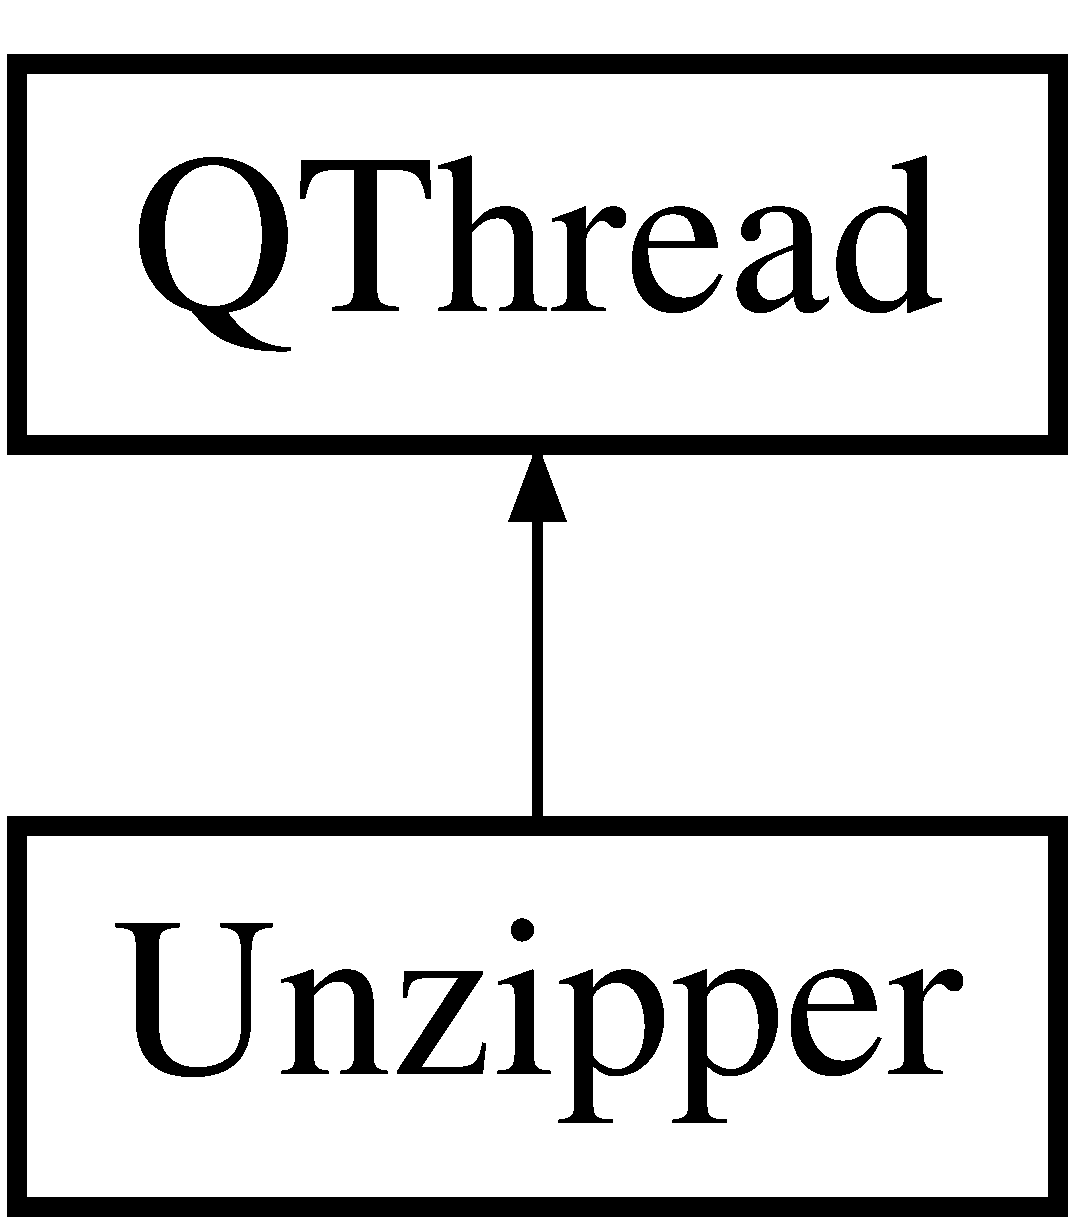
\includegraphics[height=2.000000cm]{class_unzipper}
\end{center}
\end{figure}
\subsection*{Fonctions membres publiques}
\begin{DoxyCompactItemize}
\item 
\hyperlink{class_unzipper_aace9b35fcb8e538366ed1ca6d674daec}{Unzipper} (\hyperlink{class_data_pool}{Data\+Pool}$<$ \hyperlink{class_data_buffer}{Data\+Buffer} $>$ \&zipped\+Files\+Pool, \hyperlink{class_data_pool}{Data\+Pool}$<$ \hyperlink{class_data_buffer}{Data\+Buffer} $>$ \&unzipped\+Files\+Pool)
\begin{DoxyCompactList}\small\item\em \hyperlink{class_unzipper}{Unzipper} Constructeur de la classe. \end{DoxyCompactList}\item 
\hypertarget{class_unzipper_a944444cb50d895056181adb856841def}{virtual void {\bfseries run} ()}\label{class_unzipper_a944444cb50d895056181adb856841def}

\end{DoxyCompactItemize}


\subsection{Description détaillée}
La classe \hyperlink{class_unzipper}{Unzipper} récupère des données compressées d'un \hyperlink{class_data_pool}{Data\+Pool}, les décompresse et les ajoute à un second \hyperlink{class_data_pool}{Data\+Pool}. 

\subsection{Documentation des constructeurs et destructeur}
\hypertarget{class_unzipper_aace9b35fcb8e538366ed1ca6d674daec}{\index{Unzipper@{Unzipper}!Unzipper@{Unzipper}}
\index{Unzipper@{Unzipper}!Unzipper@{Unzipper}}
\subsubsection[{Unzipper}]{\setlength{\rightskip}{0pt plus 5cm}Unzipper\+::\+Unzipper (
\begin{DoxyParamCaption}
\item[{{\bf Data\+Pool}$<$ {\bf Data\+Buffer} $>$ \&}]{zipped\+Files\+Pool, }
\item[{{\bf Data\+Pool}$<$ {\bf Data\+Buffer} $>$ \&}]{unzipped\+Files\+Pool}
\end{DoxyParamCaption}
)}}\label{class_unzipper_aace9b35fcb8e538366ed1ca6d674daec}


\hyperlink{class_unzipper}{Unzipper} Constructeur de la classe. 


\begin{DoxyParams}{Paramètres}
{\em zipped\+Files\+Pool} & \hyperlink{class_data_pool}{Data\+Pool} de données compressées \\
\hline
{\em unzipped\+Files\+Pool} & \hyperlink{class_data_pool}{Data\+Pool} de données décompressées \\
\hline
\end{DoxyParams}


La documentation de cette classe a été générée à partir des fichiers suivants \+:\begin{DoxyCompactItemize}
\item 
unzipper.\+h\item 
unzipper.\+cpp\end{DoxyCompactItemize}

\hypertarget{class_writer}{\section{Référence de la classe Writer}
\label{class_writer}\index{Writer@{Writer}}
}


La classe \hyperlink{class_writer}{Writer} écrit un fichier .ecf à partir d'un \hyperlink{class_data_pool}{Data\+Pool} de donées compressées.  




{\ttfamily \#include $<$writer.\+h$>$}

Graphe d'héritage de Writer\+:\begin{figure}[H]
\begin{center}
\leavevmode
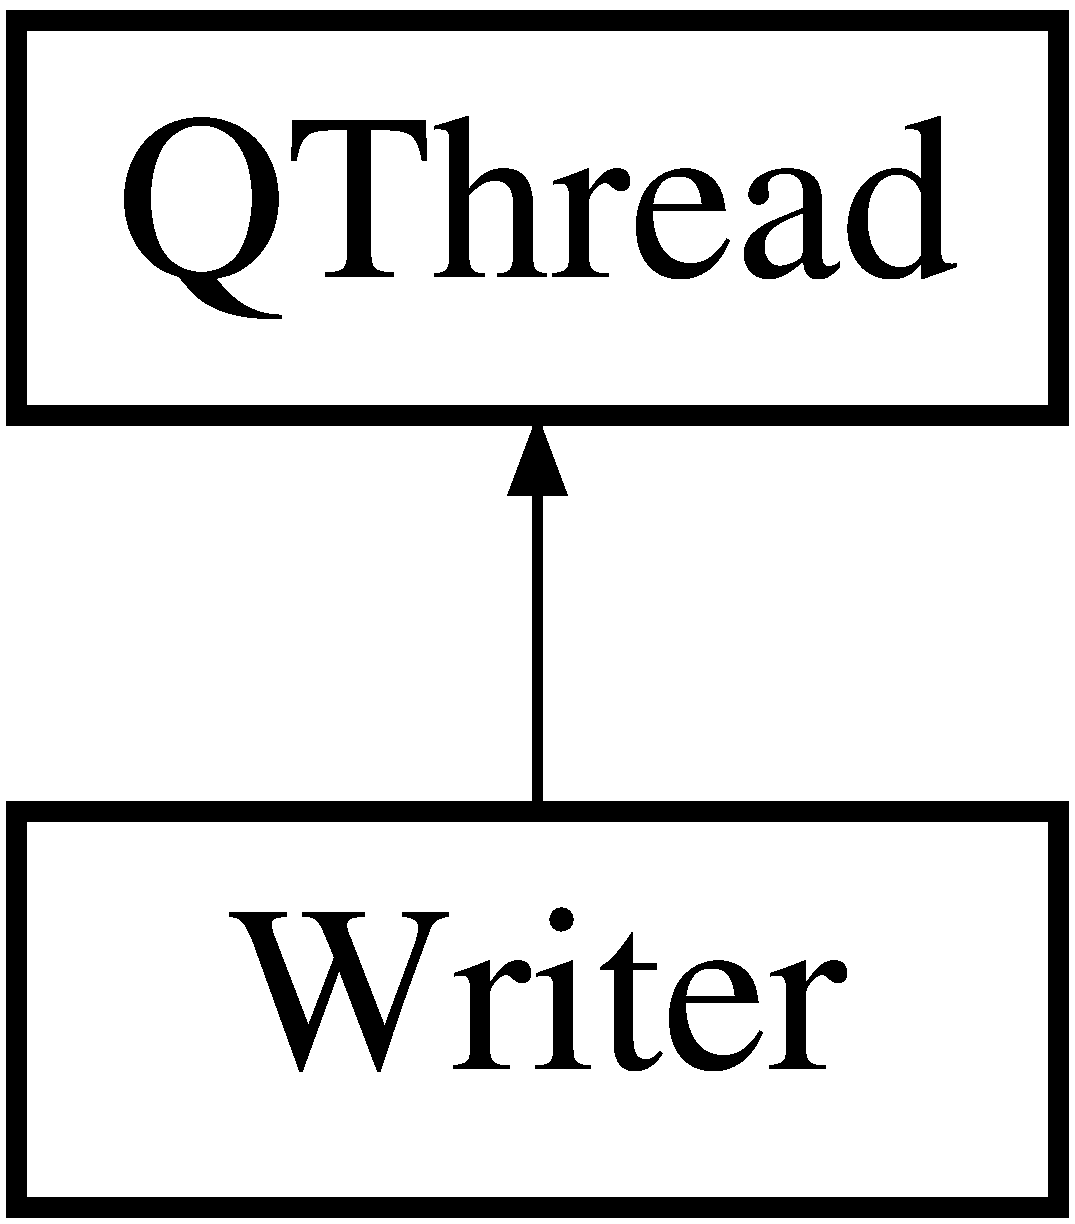
\includegraphics[height=2.000000cm]{class_writer}
\end{center}
\end{figure}
\subsection*{Fonctions membres publiques}
\begin{DoxyCompactItemize}
\item 
\hyperlink{class_writer_a02f7fe50cb56bb1bc76c7dcd399e8f38}{Writer} (\hyperlink{class_data_pool}{Data\+Pool}$<$ \hyperlink{class_data_buffer}{Data\+Buffer} $>$ \&zipped\+Files\+Pool, const Q\+String ecf\+File\+Name)
\begin{DoxyCompactList}\small\item\em \hyperlink{class_writer}{Writer} constructeur de la classe. \end{DoxyCompactList}\item 
\hypertarget{class_writer_a831f640296e4534fe5f31097fcb0712b}{virtual void {\bfseries run} ()}\label{class_writer_a831f640296e4534fe5f31097fcb0712b}

\end{DoxyCompactItemize}


\subsection{Description détaillée}
La classe \hyperlink{class_writer}{Writer} écrit un fichier .ecf à partir d'un \hyperlink{class_data_pool}{Data\+Pool} de donées compressées. 

\subsection{Documentation des constructeurs et destructeur}
\hypertarget{class_writer_a02f7fe50cb56bb1bc76c7dcd399e8f38}{\index{Writer@{Writer}!Writer@{Writer}}
\index{Writer@{Writer}!Writer@{Writer}}
\subsubsection[{Writer}]{\setlength{\rightskip}{0pt plus 5cm}Writer\+::\+Writer (
\begin{DoxyParamCaption}
\item[{{\bf Data\+Pool}$<$ {\bf Data\+Buffer} $>$ \&}]{zipped\+Files\+Pool, }
\item[{const Q\+String}]{ecf\+File\+Name}
\end{DoxyParamCaption}
)}}\label{class_writer_a02f7fe50cb56bb1bc76c7dcd399e8f38}


\hyperlink{class_writer}{Writer} constructeur de la classe. 


\begin{DoxyParams}{Paramètres}
{\em zipped\+Files\+Pool} & \hyperlink{class_data_pool}{Data\+Pool} de fichiers compressés \\
\hline
{\em ecf\+File\+Name} & fichier .ecf de destination \\
\hline
\end{DoxyParams}


La documentation de cette classe a été générée à partir des fichiers suivants \+:\begin{DoxyCompactItemize}
\item 
writer.\+h\item 
writer.\+cpp\end{DoxyCompactItemize}

\hypertarget{class_zipper}{\section{Référence de la classe Zipper}
\label{class_zipper}\index{Zipper@{Zipper}}
}


La classe \hyperlink{class_zipper}{Zipper} permet de compresser les données d'un \hyperlink{class_data_pool}{Data\+Pool} et de les stocker dans un second \hyperlink{class_data_pool}{Data\+Pool}.  




{\ttfamily \#include $<$zipper.\+h$>$}

Graphe d'héritage de Zipper\+:\begin{figure}[H]
\begin{center}
\leavevmode
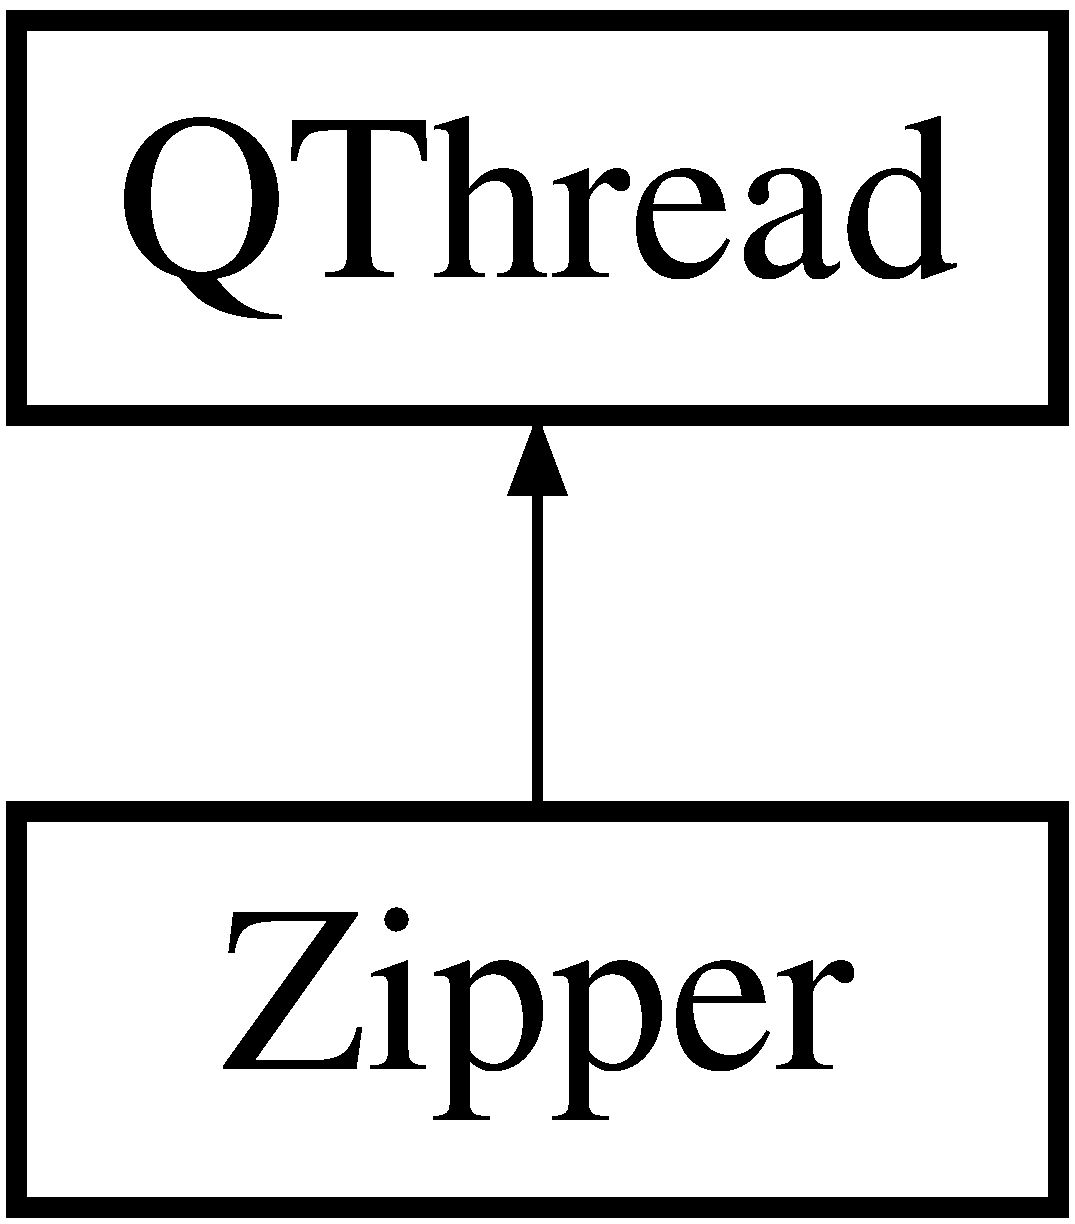
\includegraphics[height=2.000000cm]{class_zipper}
\end{center}
\end{figure}
\subsection*{Fonctions membres publiques}
\begin{DoxyCompactItemize}
\item 
\hyperlink{class_zipper_a42f9dfaa2fdf20d730c1dd5a29185353}{Zipper} (\hyperlink{class_data_pool}{Data\+Pool}$<$ Q\+String $>$ \&files\+Pool, \hyperlink{class_data_pool}{Data\+Pool}$<$ \hyperlink{class_data_buffer}{Data\+Buffer} $>$ \&zipped\+Files\+Pool, const Q\+String \&root\+Dir)
\begin{DoxyCompactList}\small\item\em \hyperlink{class_zipper}{Zipper} constructeur de la classe. \end{DoxyCompactList}\item 
\hypertarget{class_zipper_a17e7eb33d4588234dc47d24cbd0d6c09}{virtual void {\bfseries run} ()}\label{class_zipper_a17e7eb33d4588234dc47d24cbd0d6c09}

\end{DoxyCompactItemize}


\subsection{Description détaillée}
La classe \hyperlink{class_zipper}{Zipper} permet de compresser les données d'un \hyperlink{class_data_pool}{Data\+Pool} et de les stocker dans un second \hyperlink{class_data_pool}{Data\+Pool}. 

\subsection{Documentation des constructeurs et destructeur}
\hypertarget{class_zipper_a42f9dfaa2fdf20d730c1dd5a29185353}{\index{Zipper@{Zipper}!Zipper@{Zipper}}
\index{Zipper@{Zipper}!Zipper@{Zipper}}
\subsubsection[{Zipper}]{\setlength{\rightskip}{0pt plus 5cm}Zipper\+::\+Zipper (
\begin{DoxyParamCaption}
\item[{{\bf Data\+Pool}$<$ Q\+String $>$ \&}]{files\+Pool, }
\item[{{\bf Data\+Pool}$<$ {\bf Data\+Buffer} $>$ \&}]{zipped\+Files\+Pool, }
\item[{const Q\+String \&}]{root\+Dir}
\end{DoxyParamCaption}
)}}\label{class_zipper_a42f9dfaa2fdf20d730c1dd5a29185353}


\hyperlink{class_zipper}{Zipper} constructeur de la classe. 


\begin{DoxyParams}{Paramètres}
{\em files\+Pool} & \hyperlink{class_data_pool}{Data\+Pool} de fichiers non compressés \\
\hline
{\em zipped\+Files\+Pool} & \hyperlink{class_data_pool}{Data\+Pool} de fichiers compressés \\
\hline
{\em root\+Dir} & répertoire à compresser \\
\hline
\end{DoxyParams}


La documentation de cette classe a été générée à partir des fichiers suivants \+:\begin{DoxyCompactItemize}
\item 
zipper.\+h\item 
zipper.\+cpp\end{DoxyCompactItemize}

%--- End generated contents ---

% Index
\newpage
\phantomsection
\addcontentsline{toc}{chapter}{Index}
\printindex

\end{document}
